% ============================================================
% main.tex -- the "parent" file of the report.
% It only lists the parts in order. All design is in template.cls.
% Build: lualatex main -> biber main -> lualatex main -> lualatex main
% ============================================================
\documentclass{template}
\addbibresource{references.bib}

% ---------- Title page details (printed by the template) ----------
\reporttitle{דת ויציבות מדינית: האם הנצרות החלישה או חיזקה מדינות?}
           {Religion and State Stability: Did Christianity Weaken or Strengthen States?}
\reportsubtitle{מחקר השוואתי ממוחשב של רומא המערבית, רומא המזרחית והממלכה הפרנקית (\LR{312--843} לספירה)}
               {A Computational Comparative Study of Western Rome, Eastern Rome and the Frankish Kingdom (312--843 CE)}
\reporttype{דוח מכין}{Preliminary Report}
\institution{אוניברסיטת חיפה}{University of Haifa}
\course{יישומי \en{Vibe Coding} ו־\en{AI} במדע וביום־יום}
\semester{סמסטר א׳, תשפ״ז}
\authors[Liron Ben Yosef \and Yonatan Kliger]{לירון בן יוסף \and יונתן קליגר}
\lecturer{ד״ר יורם סגל}
\submissiondate{24.11.2026}
\runningtitles{דת ויציבות מדינית}{Preliminary Report}

\begin{document}

% ---------- Front matter: numbered with Hebrew letters (א, ב, ג...) ----------
\frontmatter
\makecoverpage                      % title page, no page number
% ============================================================
% chapters/00-abstract.tex -- תקציר מנהלים ומילות מפתח
% Executive summary: 250-350 words, one continuous block (booklet, sec. 2.2).
% Final version, written after all eight chapters (20.11.2026).
% Content only. The template decides where and how it is printed.
% Template must provide: environment `executivesummary`, command \keywords{...}
% ============================================================

\begin{executivesummary}
באוגוסט 410 בזזו הוויזיגותים את רומא, ומאז חוזרת השאלה אם קבלת הנצרות החלישה את הקיסרות הרומית. גיבון השיב בחיוב, ואילו רוב החוקרים בני זמננו מדגישים לחץ חיצוני, משבר כלכלי, אקלים ומגפות. לפי הטיעון המוצע בדוח, הוויכוח לא הוכרע בעיקר משום שמחקרים רבים בוחנים מקרה אחד, נשענים על דוגמאות נבחרות, ואינם מגדירים את המושגים שלהם באופן מדיד. דוח מכין זה מציע מחקר שבוחן את השאלה בהשוואה בין שלוש מדינות נוצריות שהגיעו לתוצאות שונות לגמרי: רומא המערבית, שנפלה ב־476; רומא המזרחית, שאימצה את אותה דת ושרדה עוד כאלף שנה; והממלכה הפרנקית, שהייתה נוצרית כמעט מהקמתה והתחזקה. שאלת המחקר היא אם הנצרות פעלה ככוח שמחליש או שמחזק מדינות בין המאה הרביעית למאה התשיעית, ומה קבע לאיזה כיוון היא פעלה. ההשערה המרכזית היא שהדת עצמה לא הכריעה, אלא מידת ההשתלבות בין הכנסייה לבין מוסדות המדינה. מבין שלוש חלופות שיטה נבחרה, במטריצת החלטה משוקללת, שיטה משולבת: מאגר נתונים השוואתי במקטעים של 25 שנה, שבו מדדי ההשתלבות מופקים מאלפי טקסטים עתיקים בעזרת מודלי שפה וועדת סוכני \en{AI}, ונבדקים מול תיוג של מומחה לתקופה על מדגם מבחן חתום, נפרד מקטעי הפיתוח. ניתוח רגישות הראה שהבחירה יציבה גם כשהמשקלים משתנים. המחקר נשען על כלים פתוחים קיימים – \en{Perseus}, \en{dMGH} ו־\en{Seshat} – ומוסיף להם מדידה שיטתית של היחסים בין הכנסייה למדינה. מפרט הדרישות קובע, בין היתר, שסיווגי המודל יתאימו לפחות ב־85\% לסיווג של מומחה, ושכל תוצאה תהיה ניתנת לשחזור. המחקר מתוכנן ל־12 חודשים בחמש חבילות עבודה, בתקציב תכנון של כ־111 אלף ש״ח, עם שלוש אבני דרך: תיקוף המודל בחודש החמישי, מאגר נתונים מלא בחודש השמיני, ופרסום פתוח של הקוד, הנתונים והממצאים בחודש ה־12. ארבעה סיכונים קריטיים זוהו, ובראשם הטיית המקורות שנכתבו ברובם בידי אנשי כנסייה וטעויות של מודלי השפה; לכל אחד מהם נקבעה תוכנית הפחתה, שלפי אומדן התכנון תוריד אותו מתחת לסף הקריטי. תוצרי המחקר יאפשרו לבחון את הוויכוח בן 1,600 השנים גם כשאלה אמפירית.
\end{executivesummary}

\keywords{נפילת רומא; התנצרות הקיסרות הרומית; הממלכה הפרנקית; יחסי דת ומדינה; יציבות מדינית; היסטוריה ממוחשבת; ניתוח טקסט בעזרת \en{AI}}
        % executive summary + keywords
\tableofcontents                    % automatic, down to level 3
\listoffigures
\listoftables
\input{chapters/00-abbreviations}   % abbreviations and terms

% ---------- Body: numbered 1-40 ----------
\mainmatter
% ============================================================
% chapters/01-intro.tex -- פרק 1: מבוא ורקע
% Content only. All design comes from template.cls.
% Commands used here that the template must provide:
%   \en{...}            English text inside Hebrew
%   \LR{...}            left-to-right run (year ranges)
%   keybox environment  highlighted box with a title
% ============================================================

\chapter{מבוא ורקע}
\label{ch:intro}

\section{אוגוסט 410: היום שבו רומא נבזזה}
\label{sec:intro-410}

ב־24 באוגוסט 410 נכנסו הוויזיגותים, בהנהגת המלך אלאריך, אל העיר רומא ובזזו אותה במשך שלושה ימים. היה זה הכיבוש הראשון של העיר בידי אויב זר מזה כשמונה מאות שנה, מאז פשיטת הגאלים במאה הרביעית לפני הספירה. מבחינה צבאית ומדינית, רומא כבר לא הייתה אז בירת הקיסרות: חצר הקיסר במערב ישבה ברוונה, והשלטון האמיתי התפצל מזמן בין מזרח למערב. אבל מבחינה סמלית, הזעזוע היה עצום. העיר שכבשה את העולם נכבשה בעצמה, והידיעה עברה מקצה הים התיכון ועד קצהו.

לאירוע הזה הייתה תפנית אירונית, שהיא גם נקודת המוצא של הדוח הזה: הוויזיגותים עצמם היו נוצרים. הם השתייכו לזרם האריאני, שנחשב לכפירה בעיני הכנסייה הקתולית, אבל הם כיבדו את הכנסיות של רומא כמקומות מקלט ונמנעו מלפגוע בחלק מהמסתתרים בהן \cite{augustine_citygod}. עיר נוצרית נבזזה בידי צבא נוצרי, שלושים שנה בלבד אחרי שהנצרות הוכרזה כדת הרשמית של הקיסרות.

\begin{keybox}{התקופה בקצרה}
\begin{itemize}
  \item \textbf{312} – קונסטנטינוס מנצח בקרב הגשר המילווי ומתחיל לתמוך בנצרות.
  \item \textbf{380} – תאודוסיוס הראשון קובע את הנצרות הניקאית כדת הרשמית של הקיסרות.
  \item \textbf{395} – הקיסרות מתחלקת סופית בין שני בניו של תאודוסיוס: מזרח ומערב.
  \item \textbf{410} – הוויזיגותים בוזזים את רומא.
  \item \textbf{476} – הקיסר האחרון במערב מודח; הקיסרות המזרחית ממשיכה להתקיים.
\end{itemize}
\end{keybox}

\section{ויכוח בן 1,600 שנה}
\label{sec:intro-debate}

השאלה ״האם הנצרות אשמה?״ עלתה כמעט מיד. בני העילית הפגאנית ברומא טענו שהעיר נענשה משום שזנחה את האלים שהגנו עליה במשך מאות שנים. בתגובה כתב אוגוסטינוס, הבישוף של היפו שבצפון אפריקה, את חיבורו הגדול \en{De Civitate Dei} (״עיר האלוהים״), בין השנים \LR{413--426}. אוגוסטינוס טען שגורלן של ממלכות ארציות אינו מבחן לאמת הדתית, ושמקומו האמיתי של הנוצרי הוא ״עיר האלוהים״ ולא עיר האדם \cite{augustine_citygod}.

כאלף ושלוש מאות שנה אחר כך החזיר אדוארד גיבון את הטענה הפגאנית לקדמת הבמה. בספרו \en{The History of the Decline and Fall of the Roman Empire}, שראה אור בשישה כרכים בין \LR{1776--1789}, תיאר גיבון את נפילת רומא כ״ניצחון הברבריות והדת״. לטענתו, הנצרות הסיטה את מבטם של הרומאים מן המדינה אל העולם הבא, משכה אנשים מוכשרים אל הכנסייה במקום אל הצבא והממשל, ופילגה את החברה בוויכוחים תאולוגיים \cite{gibbon_decline}.

ההיסטוריונים של העשורים האחרונים דוחים ברובם את הנצרות כהסבר מרכזי. פיטר הת'ר רואה בלחץ החיצוני של עמי הגבול, שהתחזקו דווקא בזכות מגעם הארוך עם רומא, את הגורם המכריע \cite{heather2005fall}. בריאן וורד־פרקינס מדגיש שהנפילה הייתה קטסטרופה כלכלית וחומרית אמיתית ולא ״שינוי״ שקט \cite{wardperkins2005fall}. קייל הרפר מוסיף את האקלים ואת המגפות כגורמים מרכזיים לצד תהליכים צבאיים, מדיניים וכלכליים \cite{harper2017fate}. ופיטר בראון, מגדולי חוקרי התקופה, מערער ישירות על הטענה שהעושר שזרם אל הכנסייה החליש את יכולתה של רומא לעמוד בפני הפולשים \cite{brown2012needle}.

\begin{keybox}{העובדה שמסבכת את הוויכוח}
גם הקיסרות הרומית במזרח הייתה נוצרית, ובאותה מידה כמו המערב, אבל היא שרדה עוד כאלף שנה, עד \LR{1453}. ובמערב עצמו, הממלכה הפרנקית, שהייתה נוצרית כמעט מיום הקמתה, הפכה לכוח המרכזי באירופה. אם הנצרות החלישה מדינות, איך מסבירים את שני המקרים האלה?
\end{keybox}

\section{למה עכשיו: כלים חדשים לשאלה ישנה}
\label{sec:intro-why-now}

עד לאחרונה, הוויכוח התנהל כמעט כולו בטיעונים איכותניים. מחקרים רבים התמקדו במקרה אחד ובדוגמאות שתמכו בעמדתם, והשוואה שיטתית בין מדינות שונות, באותם מדדים, הייתה קשה מאוד לביצוע. שלוש התפתחויות של השנים האחרונות משנות את המצב:

\begin{enumerate}
  \item \textbf{מאגרי נתונים היסטוריים.} מאגר \en{Seshat: Global History Databank} מקודד באופן שיטתי נתונים על מבנה חברות לאורך ההיסטוריה. מחקר שהתבסס עליו קידד נתונים על 414 חברות מ־30 אזורים ברחבי העולם, לאורך עשרת אלפים השנים האחרונות \cite{turchin2018quantitative}, ומחקר המשך בדק כמותית 17 משתנים שהוצעו בתאוריות שונות כמניעים של מורכבות חברתית \cite{turchin2022disentangling}.
  \item \textbf{ספריות טקסטים דיגיטליות.} רוב המקורות הלטיניים והיווניים של התקופה זמינים היום בפורמט דיגיטלי, וניתנים לחיפוש ולניתוח ממוחשב.
  \item \textbf{מודלי שפה.} מודלים שאומנו על טקסטים לטיניים מסוגלים לנתח שפה עתיקה; מודל \en{Latin BERT}, לדוגמה, אומן על כ־642.7 מיליון מילים לטיניות מהתקופה הקלאסית ועד ימינו \cite{bamman2020latinbert}. מודלי שפה גדולים מאפשרים לסווג אלפי קטעים לפי נושא, בהיקף שאף חוקר יחיד אינו יכול לקרוא.
\end{enumerate}

השילוב בין שלושת הכלים האלה מאפשר לבחון את הוויכוח בן 1,600 השנים גם כשאלה אמפירית: למדוד, להשוות ולבחון השערות, בהיקף ובשיטתיות שהיו קשים להשגה בעבר.

\section{המוטיבציה}
\label{sec:intro-motivation}

לשאלה יש ערך שחורג מעבר להיסטוריה של העת העתיקה. היחסים בין דת למוסדות המדינה עומדים במרכז הוויכוח הציבורי בחברות רבות גם היום, ולעתים קרובות שני הצדדים משתמשים ב״לקחי ההיסטוריה״ – ובמיוחד בנפילת רומא – כדי לתמוך בעמדתם. מחקר שמבחין בין \textbf{הדת עצמה} לבין \textbf{האופן שבו היא משתלבת במוסדות} יכול לתרום לדיון הזה בסיס עובדתי במקום אנלוגיות.

המחקר המוצע בדוח משווה שלוש מדינות נוצריות שהגיעו לתוצאות שונות לגמרי: הקיסרות הרומית המערבית, הקיסרות הרומית המזרחית והממלכה הפרנקית. ההשערה המרכזית היא שהדת כשלעצמה לא הכריעה את גורלן; מה שהכריע הוא מידת ההשתלבות בין הכנסייה לבין מוסדות המדינה.

\section{מבנה הדוח}
\label{sec:intro-structure}

פרק~\ref{ch:problem} מגדיר את הבעיה, מנסח את שאלת המחקר ואת ההשערות, ומציג את מפרט הדרישות של המחקר. פרק~\ref{ch:literature} סוקר את הספרות המחקרית לפי נושאים, מציג את מאמר הדגל ומגדיר את פער הידע. פרק~\ref{ch:market} סוקר את הכלים ומאגרי הנתונים הקיימים לחוקרי התקופה. פרק~\ref{ch:alternatives} משווה שלוש חלופות שיטה ובוחר ביניהן במטריצת החלטה משוקללת. פרק~\ref{ch:workplan} מציג את תוכנית העבודה, ופרק~\ref{ch:risks} את הסיכונים ואת דרכי ההתמודדות איתם. פרק~\ref{ch:summary} מסכם ומציג את הצעדים המיידיים לאחר אישור הדוח.

% ============================================================
% chapters/02-problem.tex -- פרק 2: הבעיה, שאלת המחקר והיעדים
% Content only. All design comes from template.cls.
% New commands used here (see work/template-needs.md):
%   table / tabular with \toprule \midrule \bottomrule (booktabs)
%   tikzpicture (figure is in figures/ch2-chain.tex)
% ============================================================

\chapter{הבעיה, שאלת המחקר והיעדים}
\label{ch:problem}

פרק זה מגדיר את מרחב הבעיה וגוזר ממנו את הדרישות של המחקר. איור~\ref{fig:problem-chain} מראה את השרשרת: מהמצב המצוי, דרך הפער, אל שאלת המחקר ואל מפרט הדרישות שלפיו ייבחן המחקר בסופו.

\begin{figure}[htbp]
  \centering
  \input{figures/ch2-chain}
  \caption{מהמצב המצוי אל מפרט הדרישות}
  \label{fig:problem-chain}
\end{figure}

\section{המצב המצוי: ויכוח בלי מדידה}
\label{sec:problem-current}

הוויכוח על תפקידה של הנצרות בנפילת הקיסרות המערבית נמשך מאז 410, אבל הוא מתנהל כמעט כולו בכלים איכותניים. כפי שהוצג בפרק~\ref{ch:intro}, גיבון ראה בנצרות גורם מחליש \cite{gibbon_decline}, ואילו חוקרים בני זמננו מדגישים את הלחץ החיצוני \cite{heather2005fall}, את הקריסה הכלכלית \cite{wardperkins2005fall} או את האקלים והמגפות \cite{harper2017fate}. לכל אחת מהעמדות יש בסיס רציני במקורות, ובכל זאת אין ביניהן הכרעה. לפי הטיעון המוצע בדוח, הסיבה העיקרית לכך אינה מחסור בידע, אלא שלוש מגבלות שיטתיות:

\begin{enumerate}
  \item \textbf{מקרה אחד בכל פעם.} רוב המחקרים שנכללו בסקירה עוסקים במערב בלבד, או במזרח בלבד, או בפרנקים בלבד. כשבוחנים מקרה אחד, אי אפשר להפריד בין השפעת הדת לבין כל שאר הגורמים שפעלו באותו מקום ובאותו זמן.
  \item \textbf{דוגמאות נבחרות.} חוקרים נוטים להביא את הדוגמאות שתומכות בטענתם. בספרות שנכללה בסקירה לא זוהתה רשימה אחידה של אירועים ומדדים שכל העמדות נבחנות מולה.
  \item \textbf{הגדרות לא מדידות.} מושגים כמו ״החלשה״, ״יציבות״ או ״השפעת הכנסייה״ נשארים עמומים. בלי הגדרה מדידה, אי אפשר לבדוק אם טענה נכונה או שגויה.
\end{enumerate}

גם הניסיונות הכמותיים הקיימים אינם עונים על השאלה. מחקרים על מאגר \en{Seshat} בודקים חברות מכל העולם ולאורך אלפי שנים, ברזולוציה גסה, ואינם מתמקדים ביחסים שבין הכנסייה למדינה \cite{turchin2018quantitative,turchin2022disentangling}. מנגד, מחקרים שמדדו את התנצרות העילית הרומית במספרים \cite{barnes1995statistics,salzman2002making} עסקו במערב בלבד, ולא קשרו את הממצאים ליציבות המדינה.

\section{הפער: שלושה מקרים, אותה דת, שלוש תוצאות}
\label{sec:problem-gap}

התקופה שבין המאה הרביעית למאה התשיעית מציעה הזדמנות נדירה למחקר השוואתי. שלוש מדינות אימצו את אותה דת, ולמרות זאת הגיעו לתוצאות הפוכות (טבלה~\ref{tab:three-cases}). מבנה כזה, שבו גורם אחד משותף לכל המקרים והתוצאה שונה, מאפשר לשאול איזה גורם \textbf{אחר} מבדיל ביניהם.

\begin{table}[htbp]
  \centering
  \caption{שלושת המקרים במחקר}
  \label{tab:three-cases}
  \begin{tabular}{p{28mm}p{28mm}p{55mm}p{29mm}}
    \toprule
    \textbf{מדינה} & \textbf{תקופה במחקר} & \textbf{הקשר לנצרות} & \textbf{התוצאה} \\
    \midrule
    רומא המערבית & \LR{312--476} & דת חדשה במוסדות ותיקים & נפלה \\
    רומא המזרחית & \LR{312--610} & אותה נקודת פתיחה & שרדה עד \LR{1453} \\
    הממלכה הפרנקית & \LR{481--843} & נוצרית כמעט מהקמתה & התחזקה, התפצלה ב־843 \\
    \bottomrule
  \end{tabular}
\end{table}

הכינויים ״מערב״ ו״מזרח״ מציינים כאן מסלולים אזוריים לצורך ההשוואה, ולא שתי מדינות עצמאיות לאורך כל התקופה. לפני חלוקת 395, וגם לאחריה באירועים בעלי תחולה משותפת, אותם שליטים ומקורות עשויים לשרת את שני המסלולים. ישויות אלה לא יטופלו כשתי חזרות עצמאיות. אירועים משותפים יסומנו בנפרד וייבחנו גם בניתוח רגישות המשמיט אותם, לפי כללי האיגום שבפרק~\ref{ch:alternatives}.

\begin{keybox}{פער הידע}
בספרות שנכללה בסקירה לא זוהה מחקר שבחן, באותם מדדים ובשיטה אחת, מה מבדיל בין שלוש מדינות נוצריות שהגיעו לתוצאות שונות. בפרט, לא זוהתה מדידה של מידת ההשתלבות בין הכנסייה למוסדות המדינה כגורם נפרד מעצם קבלת הדת.
\end{keybox}

הספרות על הפרנקים מצביעה על כיוון אפשרי. הבישופים בגאליה ניסחו אידיאלים של שלטון נוצרי עוד בעת העתיקה המאוחרת, והמלכים הפרנקים אימצו אותם \cite{moore2011sacred}; מבנה הדיוקסיות של הבישוף רמיגיוס סיפק לממלכה של כלוֹדוויג בסיס טריטוריאלי \cite{poveda2019clovis}. כלומר, אצל הפרנקים הכנסייה שימשה תשתית של המדינה. ייתכן שזה ההבדל המכריע, וייתכן שלא – וזו בדיוק השאלה שהמחקר בא לבדוק.

\section{שאלת המחקר וההשערות}
\label{sec:problem-question}

הפרויקט נשען על שאלה והשערות הניתנות לבחינה: \textbf{האם התנצרות הייתה קשורה להחלשה או לחיזוק של יציבות מדינית בשלושת מקרי המחקר, בין המאה הרביעית למאה התשיעית, ואילו מאפיינים של השתלבות הכנסייה במוסדות השלטון מבחינים בין שני הכיוונים?} השערה \en{H1} גורסת שרמת ההתנצרות כשלעצמה לא תספק הסבר יציב להבדלי היציבות לאחר התחשבות בגורמים חלופיים. השערה \en{H2} מציעה קשר חיובי בין השתלבות מוסדית של הכנסייה לבין יציבות, לעומת יחסי תחרות וסכסוך. השערת האפס \en{H0} היא שאין קשר מדיד בין מדד ההשתלבות לבין מדד היציבות בתכנון הנבדק. אי־דחיית השערת האפס לא תוכיח היעדר קשר, והפרכת \en{H2} לא תוכיח שגיבון צדק. התוצאות יפורשו לצד אי־הוודאות, הכיסוי הדל וההסברים החלופיים; המחקר התצפיתי אינו מזהה לבדו השפעה סיבתית של הדת.

\section{הגדרת המשתנים}
\label{sec:problem-variables}

כדי שההשערות יהיו ניתנות לבדיקה, כל מושג מתורגם למדדים שאפשר לאסוף מהמקורות. כל מדד נמדד בכל אחת משלוש המדינות, במקטעי זמן של 25 שנה. טבלה~\ref{tab:variables} מציגה את המדדים המוצעים.

\begin{table}[htbp]
  \centering
  \caption{המשתנים במחקר והמדדים שלהם (הצעה ראשונית)}
  \label{tab:variables}
  \begin{tabular}{p{32mm}p{62mm}p{48mm}}
    \toprule
    \textbf{משתנה} & \textbf{מדד} & \textbf{מקור הנתונים} \\
    \midrule
    \multicolumn{3}{l}{\textit{משתנה תלוי: יציבות המדינה}} \\
    & מספר ניסיונות תפיסת שלטון ומרידות & כרוניקות ותולדות \\
    & משך שלטון ממוצע של השליט & רשימות שליטים \\
    & שינוי בשטח שבשליטת המדינה & אטלסים היסטוריים, \en{Seshat} \\
    & מספר שנים של מלחמת אזרחים & כרוניקות ותולדות \\
    \midrule
    \multicolumn{3}{l}{\textit{משתנה מסביר: השתלבות כנסייה–מדינה}} \\
    & בישופים בתפקידי ממשל ושיפוט & מכתבים, החלטות מועצות \\
    & חקיקה דתית מטעם השליט & קודקסים, קפיטולריות \\
    & מועצות כנסייה שכינס השליט & פרוטוקולים של מועצות \\
    & סכסוכים גלויים בין שליט לבישופים & כרוניקות, מכתבים \\
    \midrule
    \multicolumn{3}{l}{\textit{משתנה מסביר: רמת ההתנצרות}} \\
    & שיעור העילית הנוצרית & מחקרים קיימים \cite{barnes1995statistics,salzman2002making} \\
    \midrule
    \multicolumn{3}{l}{\textit{משתני פיקוח}} \\
    & לחץ צבאי חיצוני (פלישות, קרבות) & כרוניקות, \en{Seshat} \\
    & אינדיקטורים כלכליים (מטבעות, מסים) & ממצאים ארכאולוגיים \\
    & אקלים ומגפות & מחקרי אקלים \cite{harper2017fate} \\
    \bottomrule
  \end{tabular}
\end{table}

את מדדי ההשתלבות אי אפשר לאסוף מטבלאות קיימות. הם מצויים בתוך אלפי טקסטים: מכתבים, החלטות של מועצות כנסייה, חוקים וכרוניקות. לכן חלק מרכזי במחקר הוא ניתוח של טקסטים אלה בעזרת מודלי שפה, עם תיקוף בידי מומחה (פרק~\ref{ch:alternatives}).

\section{מפרט הדרישות}
\label{sec:problem-requirements}

מפרט הדרישות הוא החוזה שלפיו ייבחן המחקר. לכל דרישה יש מזהה, ערך יעד ושיטת אימות (טבלה~\ref{tab:requirements}). דרישה בלי שיטת בדיקה היא משאלה, ולכן אף דרישה כאן אינה נשארת בלי דרך לבדוק אותה.

\begin{table}[htbp]
  \centering
  \caption{מפרט הדרישות של המחקר}
  \label{tab:requirements}
  \small
  \begin{tabular}{p{29mm}p{32mm}p{44mm}p{37mm}}
    \toprule
    \textbf{מזהה} & \textbf{הדרישה} & \textbf{ערך יעד} & \textbf{אימות} \\
    \midrule
    \en{REQ-DATA-01} & כיסוי מאגר הנתונים & 34 מקטעים לפחות, 12 משתנים בכל אחד & בדיקת שלמות אוטומטית \\
    \en{REQ-DATA-02} & תיעוד מקור לכל ערך & 100\% מהערכים & בדיקת שדות מלאה וביקורת תוכן מדגמית \\
    \en{REQ-TXT-01} & גודל קורפוס הטקסטים & 2,000 קטעים מתויגים לפחות & ספירה במאגר \\
    \en{REQ-AI-01} & דיוק הסיווג של המודל & התאמה של 85\% לפחות לתיוג מומחה & מדגם של 300 קטעים \\
    \en{REQ-AI-02} & עקביות המודל & שינוי של עד 5\% בין שתי הרצות & הרצה חוזרת על אותו מדגם \\
    \en{REQ-STAT-01} & בדיקת ההשערות & מובהקות 0.05, דיווח על גודל האפקט & סקריפט ניתוח פתוח \\
    \en{REQ-REP-01} & יכולת שחזור & כל התוצאות משוחזרות מהקוד והנתונים & הרצה נקייה במחשב אחר \\
    \bottomrule
  \end{tabular}
\end{table}

מספר המקטעים בדרישה \en{REQ-DATA-01} נגזר מהתקופות שבטבלה~\ref{tab:three-cases}: כ־7 מקטעים של 25 שנה במערב, כ־12 במזרח וכ־15 אצל הפרנקים.

\subsection*{אילוצים}

\begin{itemize}
  \item \textbf{זמן:} 12 חודשי עבודה, צוות של שני חוקרים.
  \item \textbf{שפות המקורות:} לטינית ויוונית. התרגום והסיווג נעשים בעזרת מודלי שפה, ומחייבים תיקוף אנושי.
  \item \textbf{שרידות המקורות:} רוב הטקסטים ששרדו נכתבו בידי אנשי כנסייה. הטיה זו מטופלת בפרק~\ref{ch:risks}.
  \item \textbf{עלות:} ניתוח אלפי טקסטים במודלי שפה כרוך בעלות של טוקנים, שתוגבל בתקציב מוגדר מראש.
\end{itemize}

% ============================================================
% chapters/03-literature.tex -- פרק 3: סקירת ספרות ומאמר הדגל
% Content only. All design comes from template.cls.
% New commands used here (see work/template-needs.md):
%   \checkmark (amssymb) in the literature matrix
%   figure in figures/ch3-flagship.tex
% ============================================================

\chapter{סקירת ספרות ומאמר הדגל}
\label{ch:literature}

הסקירה בפרק זה בנויה לפי נושאים ולא לפי סדר כרונולוגי. בכל נושא מוצגים הטענה, הבסיס לה ומגבלותיה, ובסוף הפרק מרוכזים הממצאים במטריצת ספרות שמראה היכן נמצא הפער. סעיפים~\LR{\ref{sec:lit-classic}--\ref{sec:lit-wealth}} עוסקים בשאלת נפילת המערב, סעיפים~\LR{\ref{sec:lit-east}--\ref{sec:lit-franks}} בשני המקרים המשווים, סעיף~\ref{sec:lit-computational} בשיטות הכמותיות שהמחקר נשען עליהן, וסעיפים~\LR{\ref{sec:lit-models}--\ref{sec:lit-method-issues}} מחברים את הממצאים לדגמים ולקשיים מתודולוגיים.

\section{ההסבר הדתי הקלאסי: מאוגוסטינוס ועד גיבון}
\label{sec:lit-classic}

הטענה שהנצרות אחראית לחולשת רומא קדומה כמעט כמו האירועים עצמם. אחרי הביזה של 410 האשימו בני העילית הפגאנית את הנוצרים בכך שהעיר נטשה את האלים שהגנו עליה, ואוגוסטינוס כתב את ״עיר האלוהים״ כדי להשיב להם \cite{augustine_citygod}. אוגוסטינוס אינו רואה בהצלחה של ממלכה ארצית הוכחה לאמיתות הדת. עם זאת, אין להסיק מכך שלדעתו הנצרות אינה מועילה לחיים המדיניים: הוא דן במעלות של שליטים נוצרים ובשלום הארצי המשותף לקבוצות שונות (ספר ה, פרקים \LR{24--26}; ספר יט, פרק 17). ההבחנה היא בין טובת המדינה לבין אמת דתית, ולא שלילה גורפת של תועלת אזרחית.

אדוארד גיבון הפך את הטענה הפגאנית לתזה היסטורית שיטתית. לפי גיבון, הנצרות הפנתה את תשומת הלב מן המדינה אל העולם הבא, הפנתה את המוכשרים אל הכנסייה במקום אל הצבא והממשל, ופילגה את הקיסרות בוויכוחים תאולוגיים \cite{gibbon_decline}. יש להבחין בין ביקורתו של גיבון לבין טענה חד־סיבתית פשוטה. בפרק 38 הוא עצמו מתייחס להישרדות המזרח, ואף מייחס לנצרות תפקיד בריכוך אלימות הפולשים לצד תרומתה לחולשת האימפריה. לכן המזרח אינו מקרה שגיבון התעלם ממנו. מגבלת הטיעון לצורך המחקר הנוכחי היא היעדר מבחן השוואתי כמותי לפי מדדים אחידים, ולא היעדר מודעות להסברים מנוגדים.

\section{לחץ חיצוני, כלכלה והגישה ״הקטסטרופלית״}
\label{sec:lit-external}

במחקר של העשורים האחרונים, ההסבר הדתי נדחק הצידה לטובת הסברים חיצוניים וכלכליים. פיטר הת'ר טוען שהקיסרות במאה הרביעית לא הייתה על סף קריסה פנימית. לדעתו, מאות שנות מגע עם רומא שינו את העמים שמעבר לגבול והפכו אותם לאויב מאורגן וחזק בהרבה; לחץ ההונים דחף את הגותים ואחרים אל תוך הקיסרות, ושני דורות של מאבקים שברו את המערב \cite{heather2005fall}. בריאן וורד־פרקינס, שספרו יצא באותה שנה, מתווכח עם הגישה שרואה בסוף העת העתיקה ״שינוי״ הדרגתי ושקט. הוא מצביע על ממצאים ארכאולוגיים שמראים ירידה חדה ברמת החיים החומרית במערב, ורואה בנפילה קטסטרופה אמיתית \cite{wardperkins2005fall}.

שתי העבודות חשובות למחקר המוצע משום שהן מספקות את \textbf{משתני הפיקוח}: אם רוצים לבדוק את השפעת הדת, צריך קודם להביא בחשבון את הלחץ הצבאי ואת המצב הכלכלי. בנוסף, כריס ויקהאם השווה באופן שיטתי בין אזורים שונים באירופה ובאגן הים התיכון בין 400 ל־800 \cite{wickham2005framing}, והראה שהשוואה בין אזורים היא כלי רב עוצמה להבנת התקופה. המגבלה המשותפת לעבודות האלה, מנקודת המבט של המחקר המוצע, היא שהן אינן עוסקות בדת כמשתנה עצמאי. הן מסבירות את הנפילה בלעדיה, אבל לא בודקות אותה.

\section{אקלים ומגפות}
\label{sec:lit-climate}

קייל הרפר הוסיף לוויכוח ממד שכמעט לא נבחן לפניו. בעזרת נתוני אקלים, ממצאים גנטיים ומקורות כתובים, הוא מציג שינויי אקלים ומגפות כגורמים מרכזיים במשברי האימפריה, לצד החלטות ותהליכים אנושיים. הצגה זו אינה אומדן כמותי של חלוקת האחריות בין סביבה, מחלות ובני אדם \cite{harper2017fate}.

לעבודה של הרפר שתי השלכות על המחקר המוצע. ראשית, היא מוסיפה משתנה פיקוח שלישי, סביבתי. שנית, היא מראה שאפשר לשלב נתונים כמותיים מתחומי מדע אחרים בשאלה היסטורית ״קלאסית״, וזה בדיוק סוג השילוב שהמחקר המוצע מציע.

\section{הכנסייה, העושר והעילית הרומית}
\label{sec:lit-wealth}

הדיון המעמיק ביותר בקשר שבין הנצרות לבין מוסדות המדינה מתנהל סביב העילית הרומית. בשנת 1961 הציע פיטר בראון מודל להבנת התהליך שבו האריסטוקרטיה של רומא הפכה לנוצרית במהלך המאות הרביעית והחמישית \cite{brown1961aspects}. שלושה עשורים אחר כך ניסה ט״ד בארנס לבחון את התהליך הזה \textbf{סטטיסטית}, וטען שהאריסטוקרטיה התנצרה מוקדם משמעותית ממה שהניחו בראון ורוב החוקרים \cite{barnes1995statistics}. מישל זלצמן הרחיבה את הגישה הכמותית ובנתה מאגר של 414 אריסטוקרטים מהשנים \LR{284--423} שזיקתם הדתית ידועה. לפי ממצאיה, העילית התנצרה משום שהנצרות הותאמה לתרבות המעמד של האליטה הקיסרית \cite{salzman2002making}.

שלוש העבודות האלה הן התקדים הישיר לשיטה המוצעת: הן מראות שאפשר \textbf{למדוד} התנצרות, ולא רק לתאר אותה. אבל כולן עוסקות במערב בלבד, ואף אחת מהן אינה קושרת את קצב ההתנצרות ליציבות המדינה.

בעבודה מאוחרת יותר שלו, ״דרך חור המחט״, חוזר בראון לשאלה שהעסיקה את גיבון ועונה עליה באופן הפוך. הוא בוחן את היחס לעושר בנצרות המערבית בין 350 ל־550, דרך כתביהם של אמברוזיוס, אוגוסטינוס, ירונימוס ואחרים, ומערער על הרעיון הנפוץ שהעושר שזרם אל הכנסייה החליש את יכולתה של רומא לעמוד בפני הפולשים \cite{brown2012needle}. זהו אולי העימות הישיר ביותר עם גיבון בספרות המודרנית.

רובין ווילן מוסיף נקודת מבט חשובה: לא הכנסייה מול המדינה, אלא הנוצרים \textbf{בתוך} המדינה. במאמר שפורסם ב־\en{Journal of Roman Studies} הוא בוחן מכתבים של אנשי כנסייה לפקידים קיסריים, ומראה שעד המחצית הראשונה של המאה החמישית התפתחה ברחבי הים התיכון רטוריקה נוצרית של כהונה בתפקיד ציבורי \cite{whelan2018mirrors}. בספר חדש הוא מרחיב את הטענה וטוען שמי ששירתו את המדינה בעת העתיקה המאוחרת יכלו להיחשב, ולראות את עצמם, כבעלי סמכות נוצרית \cite{whelan2026serving}. הספר כולל פרק שמשווה במפורש בין מזרח למערב, ולכן הוא רלוונטי במיוחד למחקר המוצע. העבודות של ווילן מחזקות את ההנחה שבבסיס \en{H2}: מה שחשוב אינו אם המדינה נוצרית, אלא \textbf{איך} הנצרות נכנסה למנגנון שלה.

\section{למה המזרח שרד}
\label{sec:lit-east}

רבים מהדיונים על ״נפילת רומא״ שוכחים שרק החצי המערבי של הקיסרות נפל. סטיבן ויליאמס וג'רארד פריל מקדישים את ספרם לשאלה מדוע המזרח שרד את המאה החמישית. לטענתם, המזרח אימץ אסטרטגיות חדשות ומוצלחות – דיפלומטיות, צבאיות, פוליטיות ופיסקליות – שיצרו מדינה ריכוזית חדשה בקונסטנטינופול \cite{williams1999rome}.

מנקודת המבט של המחקר המוצע, המזרח הוא ״מקרה הביקורת״ החשוב ביותר: אותה דת, אותו מוצא מוסדי, ותוצאה הפוכה. ההסברים שמציעים ויליאמס ופריל הם בעיקר צבאיים, כלכליים וגיאוגרפיים, ותפקידה של הכנסייה כמעט אינו נבחן אצלם כגורם נפרד. כאן נמצא אחד הפערים שהמחקר המוצע מבקש לסגור.

\section{הכנסייה והמלכות אצל הפרנקים}
\label{sec:lit-franks}

המקרה הפרנקי מציג תמונה כמעט הפוכה לזו של המערב הרומי. כאן הכנסייה לא נוספה למוסדות ותיקים, אלא השתתפה בבנייתם.

\paragraph{ראשית הממלכה.} אחד המקורות הבודדים מימי שלטונו של כלוֹדוויג הוא מכתב שכתב לו רמיגיוס, הבישוף של ריימס, ובו הוא מייעץ למלך הצעיר כיצד לשלוט. גרהאם בארט וג'ורג' וודהויסן מציעים קריאה חדשה של המכתב, ואף מתקנים את המסורת המקובלת לגבי מועדו ומשמעותו \cite{barrett2016remigius}. פבלו פובדה אריאס בוחן את הברית בין שני האישים ומראה שהיא נבעה מצורכי ההישרדות הפוליטית של שניהם. לטענתו, מבנה הדיוקסיות של רמיגיוס סיפק לממלכה החדשה \textbf{בסיס טריטוריאלי} – כלומר, הכנסייה שימשה תשתית של המדינה. אבל המאמר מוסיף ניואנס חשוב: היחסים נשחקו עם הזמן, כשהבישוף החל לחשוש מכוחו הגובר של המלך \cite{poveda2019clovis}.

\paragraph{המלכות הנוצרית.} מייקל מור מתאר את המלכות הנוצרית אצל הפרנקים כתוצאה של השפעה הדדית בין מלכים לבישופים. לדבריו, המלכים אימצו אידיאלים שהבישופים ניסחו כבר בעת העתיקה המאוחרת, בעיקר דרך מועצות הכנסייה \cite{moore2011sacred}. ג'נט נלסון הראתה, כבר במאמר מוקדם, את הקשר בין סינודים ארציים, תפיסת המלכות כמשרה ומשיחת המלך \cite{nelson1971synods}. הספר של מרקוס קוסטמביס, מתיו אינס וסיימון מקלין מסכם את המחקר העדכני על העולם הקרולינגי, ומקדיש פרקים נפרדים לאמונה ולתרבות ולפוליטיקה ולממשל לפני 840 ואחריו \cite{costambeys2011carolingian}.

\paragraph{כשהשילוב הופך למתח.} השילוב בין הכנסייה למלכות לא היה תמיד יציב. מאייקה דה יונג מנתחת את שלטונו של לואי החסיד, בנו של קרל הגדול, שב־833, אחרי מרד של שלושת בניו הבכורים, נאלץ לעבור כפרה פומבית שהייתה למעשה הדחה. לטענתה, הכפרה הזו נבעה משיח פוליטי שבו האחריות של השליט כלפי אלוהים הפכה למרכזית \cite{dejong2009penitential}. כלומר, אותו שילוב שחיזק את המלכות יצר גם כלי להחלשתה. נלסון בוחנת את המתח הזה גם אחרי חלוקת הקיסרות, בתקופת שלטונו של שארל הקירח \cite{nelson1991bailiffs}.

\paragraph{קול ביקורתי.} קונור אובריאן מציע לקרוא את התקופה אחרת. לטענתו, המלכות הנוצרית לא צמחה ממאבק של ״כנסייה מול מדינה״, וגם לא מניצול מחושב של הדת בידי שליטים, אלא מחיפוש אחר שלטון טוב \cite{obrien2026rise}. הטענה הזו היא אתגר חשוב למחקר המוצע, משום שהמדדים המוצעים מניחים שאפשר להבחין בין ״כנסייה״ לבין ״מדינה״. סוגיה זו נידונה בניתוח הסיכונים (פרק~\ref{ch:risks}).

\section{היסטוריה ממוחשבת וניתוח טקסטים ב־\en{AI}}
\label{sec:lit-computational}

בעשור האחרון התפתח תחום שבוחן שאלות היסטוריות גדולות בכלים כמותיים. מאגר \en{Seshat} מרכז נתונים מקודדים על חברות לאורך ההיסטוריה. במחקר שפורסם ב־\en{PNAS} קודדו נתונים על 414 חברות מ־30 אזורים לאורך עשרת אלפים שנה, ונמצא שמאפיינים שונים של מורכבות חברתית קשורים זה לזה בחוזקה: רכיב אחד מסביר כשלושה רבעים מהשונות \cite{turchin2018quantitative}. מחקר המשך בדק 17 משתנים מנבאים, שמייצגים את התאוריות המרכזיות על התפתחות המורכבות החברתית, ויותר ממאה אלף צירופים שלהם \cite{turchin2022disentangling}.

במקביל התפתחו כלים לניתוח ממוחשב של שפות עתיקות. דייוויד במן ופטריק ברנס פיתחו את \en{Latin BERT}, מודל שפה שאומן על כ־642.7 מיליון מילים לטיניות, והראו שהוא משפר משימות כמו תיוג חלקי דיבר וחיפוש סמנטי \cite{bamman2020latinbert}. הגרסה המצוטטת היא קדם־פרסום ב־\en{arXiv}, ולכן הוא משמש בדוח כהדגמה לאפשרויות הטכנולוגיות ולא כבסיס מתודולוגי.

מחקרים שפיטים מהשנים האחרונות מראים שהכלים האלה הבשילו. סקירה מקיפה שפורסמה ב־\en{Computational Linguistics} ממפה את המחקר שהשתמש בלמידת מכונה לחקר טקסטים עתיקים בכל שפה, כתב ומדיום, ומתארת כיצד הכלים האלה מאפשרים ניתוח בהיקף ובפירוט שמשנים את מדעי הרוח \cite{sommerschield2023survey}. הדוגמה הבולטת היא \en{Ithaca}, רשת נוירונים שאומנה לשחזר כתובות יווניות פגומות, לזהות את מקום כתיבתן ולתארך אותן, ופורסמה ב־\en{Nature}. במבחן שחזור של חסרים שהוסתרו בכתובות יווניות, דיוק המודל היה כ־62\%; היסטוריונים ללא הכלי הגיעו לכ־25\%, ובסיועו לכ־72\% \cite{assael2022ithaca}. יישום פילולוגי נוסף הוא פרויקט \en{Logion}, המשתמש בלמידת מכונה כדי להשלים פערים בטקסטים, לזהות שגיאות של מעתיקים ולהציע תיקונים \cite{graziosi2023philology}.

המסקנה מהמחקרים האלה חשובה לתכנון המחקר: מודל השפה אינו מחליף את ההיסטוריון, אלא עובד לצידו. תוצאות אלה מצדיקות לבדוק סיוע של מודל למומחה, אך אינן מבטיחות יתרון בכל משימה ואינן מודדות את דיוק הסיווג המוצע כאן. לכן מפרט הדרישות (פרק~\ref{ch:problem}) מחייב תיקוף של סיווגי המודל בידי מומחה, ולא מסתפק בתוצאות המודל עצמו.

\section{שלושה דגמים של יחסי כנסייה–מדינה}
\label{sec:lit-models}

כשמחברים את הספרות על שלושת המקרים, מתקבלת תמונה של שלושה דגמים שונים של יחסים בין הכנסייה למדינה (טבלה~\ref{tab:three-models}). חשוב להדגיש שהטבלה מסכמת את מה שהספרות מציעה; היא אינה ממצא מחקרי, אלא נקודת המוצא שהמחקר המוצע בא לבדוק.

\begin{table}[htbp]
  \centering
  \caption{שלושה דגמים של יחסי כנסייה–מדינה, לפי הספרות}
  \label{tab:three-models}
  \small
  \begin{tabular}{p{26mm}p{42mm}p{42mm}p{30mm}}
    \toprule
    \textbf{מקרה} & \textbf{מה הספרות מתארת} & \textbf{מה זה מציע לגבי \en{H2}} & \textbf{מקורות עיקריים} \\
    \midrule
    רומא המערבית & העילית התנצרה בתוך מוסדות ותיקים; ויכוח פתוח על השאלה אם העושר שעבר לכנסייה החליש את המדינה & הכנסייה כמוסד מקביל – אבל בראון מערער על כך & \cite{gibbon_decline,brown2012needle,salzman2002making} \\
    \midrule
    רומא המזרחית & מדינה ריכוזית שאימצה אסטרטגיות חדשות במאה החמישית; פקידים נוצרים בתוך המנגנון הקיסרי & השתלבות בתוך מדינה חזקה & \cite{williams1999rome,whelan2018mirrors,whelan2026serving} \\
    \midrule
    הממלכה הפרנקית & הבישופים סיפקו בסיס טריטוריאלי ואידיאלים של שלטון; המלכות נבנתה יחד עם הכנסייה & הכנסייה כתשתית של המדינה – אבל גם כמקור למתח & \cite{poveda2019clovis,moore2011sacred,dejong2009penitential} \\
    \bottomrule
  \end{tabular}
\end{table}

הדגם הזה מעורר שאלה מעניינת. ווילן מצא רטוריקה נוצרית של כהונה ציבורית במכתבים של אוגוסטינוס, שכתב במערב, לצד מכתבים של איזידורוס מפלוסיון ותאודורטוס מקירוס, שכתבו במזרח \cite{whelan2018mirrors}. כלומר, האידיאל של ״פקיד נוצרי״ התקיים בשני חלקי הקיסרות. אם כך, ההבדל בין המזרח למערב אינו יכול לנבוע מהאידיאל עצמו, אלא מהאופן שבו הוא יושם בתוך מוסדות בעלי עוצמה שונה. זו בדיוק ההבחנה שהמדדים המוצעים (פרק~\ref{ch:problem}) מנסים לתפוס.

\section{סוגיות מתודולוגיות שעולות מהספרות}
\label{sec:lit-method-issues}

מעבר לטענות עצמן, הספרות מלמדת על שלושה קשיים שכל מחקר בתחום צריך להתמודד איתם.

\paragraph{מה נחשב ״נפילה״?} הוויכוח בין וורד־פרקינס לבין הגישה שרואה בתקופה ״שינוי״ הדרגתי \cite{wardperkins2005fall} אינו רק ויכוח על עובדות, אלא גם על הגדרות. אם הנפילה היא קטסטרופה, צריך למדוד את עומק הנזק; אם היא שינוי, צריך למדוד את קצב המעבר. לכן המחקר המוצע אינו מגדיר ״נפילה״ כאירוע אחד, אלא מודד יציבות לאורך זמן בכמה מדדים נפרדים (טבלה~\ref{tab:variables}).

\paragraph{מי כתב את המקורות?} רוב הטקסטים ששרדו מהתקופה נכתבו בידי אנשי כנסייה. המכתב של רמיגיוס לכלוֹדוויג, למשל, הוא מן המקורות הבודדים בני הזמן משלטונו \cite{barrett2016remigius}, ותולדות הפרנקים נכתבו בידי בישופים. מקורות כאלה נוטים להציג את הכנסייה בתפקיד מרכזי, וכל מדידה שמבוססת עליהם עלולה להגזים בחשיבותה. נטפל בהטיה זו בפרק~\ref{ch:risks}.

\paragraph{המספרים רגישים להנחות.} הוויכוח בין בראון לבין בארנס על מועד התנצרות העילית הרומית \cite{brown1961aspects,barnes1995statistics} מראה ששני חוקרים מעולים יכולים להגיע למסקנות שונות מאותם מקורות, בהתאם לאופן שבו הם מגדירים ״נוצרי״ ומי נכלל במדגם. המסקנה עבורנו היא שכל מדד חייב הגדרה מפורשת ומתועדת, וניתוח רגישות שבודק מה קורה כשההגדרה משתנה.

\section{מטריצת הספרות}
\label{sec:lit-matrix}

טבלה~\ref{tab:lit-matrix} מרכזת את המקורות המרכזיים לפי הנושאים שבהם הם עוסקים. כל שורה היא מקור, וכל עמודה היא נושא; סימן \checkmark{} מציין שהמקור עוסק בנושא באופן מהותי. המשבצות הריקות מסמנות את הפער.

\begin{table}[htbp]
  \centering
  \caption{מטריצת הספרות: המקורות המרכזיים מול נושאי המחקר}
  \label{tab:lit-matrix}
  \small
  \begin{tabular}{p{30mm}*{6}{>{\centering\arraybackslash}p{17mm}}}
    \toprule
    \textbf{מקור} & \textbf{דת כגורם} & \textbf{כלכלה וצבא} & \textbf{מזרח מול מערב} & \textbf{פרנקים} & \textbf{שיטה כמותית} & \textbf{קריאת מקורות} \\
    \midrule
    גיבון \cite{gibbon_decline}             & \checkmark & \checkmark & & & & \\
    הת'ר \cite{heather2005fall}             & & \checkmark & & & & \\
    וורד־פרקינס \cite{wardperkins2005fall}  & & \checkmark & & & & \\
    הרפר \cite{harper2017fate}              & & \checkmark & & & \checkmark & \\
    בראון \cite{brown2012needle}            & \checkmark & \checkmark & & & & \checkmark \\
    זלצמן \cite{salzman2002making}          & \checkmark & & & & \checkmark & \\
    ווילן \cite{whelan2026serving}          & \checkmark & & \checkmark & & & \checkmark \\
    ויליאמס ופריל \cite{williams1999rome}  & & \checkmark & \checkmark & & & \\
    מור \cite{moore2011sacred}              & \checkmark & & & \checkmark & & \\
    פובדה אריאס \cite{poveda2019clovis}     & \checkmark & & & \checkmark & & \checkmark \\
    טורצ'ין ואחרים \cite{turchin2022disentangling} & & \checkmark & & & \checkmark & \\
    אסאל ואחרים \cite{assael2022ithaca}     & & & & & \checkmark & \checkmark \\
    \midrule
    \textbf{המחקר המוצע}                    & \checkmark & \checkmark & \checkmark & \checkmark & \checkmark & \checkmark \\
    \bottomrule
  \end{tabular}
\end{table}

המטריצה מראה שני דברים. הראשון: אף אחד מהמקורות שבמטריצה אינו משווה בין שלושת המקרים – המערב, המזרח והפרנקים. השני: העבודות שעוסקות בדת כגורם אינן כמותיות (למעט זלצמן, שעוסקת בתהליך ההתנצרות ולא בהשלכותיו על המדינה), והעבודות הכמותיות אינן מתמקדות בדת. המחקר המוצע נמצא בדיוק בחיתוך הזה.

\section{מאמר הדגל}
\label{sec:lit-flagship}

מאמר הדגל הוא הפרסום שממנו המחקר שואב את הבסיס המתודולוגי הישיר ביותר. שלושה קריטריונים קובעים את הבחירה (איור~\ref{fig:flagship}): פרסום בבמה שפיטה בעלת דירוג גבוה; קרבה ישירה לבעיה, כך שהשיטה של המאמר משמשת בסיס לשיטה המוצעת; ושקיפות שמאפשרת לחזור על התוצאות, עם מדדים כמותיים.

\begin{figure}[htbp]
  \centering
  \input{figures/ch3-flagship}
  \caption{מאמר הדגל נמצא בחיתוך של שלושת הקריטריונים}
  \label{fig:flagship}
\end{figure}

על פי הקריטריונים האלה נבחר המאמר של טורצ'ין ושותפיו שפורסם ב־\en{Science Advances} בשנת 2022 \cite{turchin2022disentangling}:

\begin{itemize}
  \item \textbf{במה שפיטה:} \en{Science Advances} הוא כתב עת שפיט ומוביל של האגודה האמריקנית לקידום המדע.
  \item \textbf{קרבה לבעיה:} המאמר עושה בדיוק את מה שהמחקר המוצע מבקש לעשות – הוא בודק כמה הסברים מתחרים \textbf{בבת אחת}, על אותם נתונים, ומכריע ביניהם סטטיסטית. החוקרים בנו מודל דינמי ובדקו בעזרתו 17 משתנים שמייצגים תאוריות שונות, ויותר ממאה אלף צירופים שלהם.
  \item \textbf{חזרתיות:} המחקר מבוסס על מאגר \en{Seshat}, שהנתונים בו מתועדים ונגישים לחוקרים.
\end{itemize}

הממצא המרכזי של המאמר הוא שהשילוב בין עלייה בתפוקה החקלאית לבין אימוץ טכנולוגיות צבאיות הוא ההסבר הנתמך ביותר להתפתחות המורכבות החברתית \cite{turchin2022disentangling}.

\subsection*{העקרונות הנגזרים ממאמר הדגל}

מעבר לממצא עצמו, שלושה עקרונות במאמר הם הבסיס לשיטה המוצעת. העיקרון הראשון הוא \textbf{מבחן בין הסברים מתחרים}: במקום לבדוק תאוריה אחת ולחפש לה תמיכה, החוקרים הכניסו את כל ההסברים לאותו מודל ובדקו איזה מהם מסביר את הנתונים טוב יותר. במחקר המוצע יושוו הסברים מתחרים במספר משתנים מוגבל, בהתאם לגודל המדגם ולתוכנית הניתוח שבסעיף~\ref{sec:alt-statistics}. העיקרון השני הוא \textbf{בדיקה של צירופים רבים}: החוקרים לא הסתפקו במודל אחד, אלא בדקו יותר ממאה אלף צירופים של משתנים, וכך הראו שהמסקנה אינה תלויה בבחירה שרירותית. במחקר המוצע ייבחנו הגדרות חלופיות של המדדים בניתוחי רגישות מתועדים. העיקרון השלישי הוא \textbf{נתונים מתועדים ופתוחים}: כל ערך במאגר מקושר למקור שלו, וזה הבסיס לדרישה \en{REQ-DATA-02}.

\section{ניתוח מאמר הדגל ופער הידע}
\label{sec:lit-gap}

לצד החוזקות שלו, למאמר הדגל שלוש מגבלות מבחינת שאלת המחקר. ראשית, הוא בוחן חברות מכל העולם לאורך אלפי שנים, ויחידות הניתוח שלו גסות מכדי לזהות הבדלים בין מדינות שכנות באותה תקופה, כמו המזרח והמערב הרומיים. שנית, הוא עוסק בתאוריות רחבות על התפתחות המורכבות החברתית, ואינו מודד את אופן ההשתלבות של הכנסייה במוסדות המדינה. שלישית, הנתונים שלו מקודדים בידי מומחים מתוך הספרות המחקרית, ולא מתוך ניתוח ישיר של המקורות העתיקים עצמם.

\begin{keybox}{פער הידע}
בספרות שנכללה בסקירה לא זוהה מחקר שבדק, בשיטה כמותית אחת ובאותם מדדים, אם האופן שבו הכנסייה השתלבה במוסדות המדינה מסביר את ההבדל בין גורלן של רומא המערבית, רומא המזרחית והממלכה הפרנקית. המחקר המוצע מתאים את גישת ״המבחן ההשוואתי״ של מאמר הדגל לשאלה ממוקדת זו, ומוסיף לה ניתוח ישיר של הטקסטים העתיקים בעזרת מודלי שפה, עם תיקוף בידי מומחה.
\end{keybox}

\input{chapters/04-market}
% ============================================================
% chapters/05-alternatives.tex -- פרק 5: חלופות שיטה, בחירה וחדשנות
% Content only. All design comes from template.cls.
% Figures: figures/ch5-architecture.tex (TikZ),
%          figures/ch5-decision.pdf, figures/ch5-sensitivity.pdf (code/make_figures.py)
% The scores and weights in tab:decision MUST match ALTS and WEIGHTS in
% code/make_figures.py. Change both together.
% ============================================================

\chapter{חלופות שיטה, בחירת הפתרון וחדשנות}
\label{ch:alternatives}

בפרויקט מחקרי, ״חלופות התכן״ הן דרכים שונות לענות על שאלת המחקר. פרק זה מציג שלוש חלופות ששונות זו מזו בעיקרון ולא רק בפרטים, בוחר ביניהן במטריצת החלטה משוקללת, בודק אם הבחירה יציבה, ומתאר את הארכיטקטורה של החלופה שנבחרה ואת החדשנות שבה.

\section{שלוש חלופות שונות עקרונית}
\label{sec:alt-three}

\paragraph{חלופה א: מחקר מקורות קלאסי.} זו הדרך שבה נחקרה השאלה עד היום. החוקר בוחר מקורות מרכזיים מכל אחת משלוש המדינות – כרוניקות, מכתבים, חוקים והחלטות של מועצות כנסייה – קורא אותם לעומק, ומשווה ביניהם בכתיבה פרשנית. התוצר הוא חיבור טיעוני, בדומה לעבודות שנסקרו בפרק~\ref{ch:literature}.

\paragraph{חלופה ב: מאגר נתונים וקידוד ידני.} צוות של מומחים בונה מאגר נתונים לפי המשתנים שהוגדרו בפרק~\ref{ch:problem}. כל ערך במאגר נקבע בידי מומחה שקורא את המקורות הרלוונטיים ומקודד אותם לפי ספר הנחיות אחיד. זו הגישה של מאגר \en{Seshat} ושל המחקרים שמדדו את התנצרות העילית הרומית \cite{salzman2002making}. התוצר הוא מאגר מובנה, שעליו מריצים ניתוח סטטיסטי.

\paragraph{חלופה ג: מאגר נתונים וניתוח טקסט בעזרת \en{AI}, עם תיקוף מומחה.} כמו בחלופה ב, נבנה מאגר מובנה; אבל את מדדי ההשתלבות בין הכנסייה למדינה מפיק מודל שפה, שמסווג אלפי קטעים מתוך המקורות. מומחה בודק מדגם מתוך הסיווגים, ורק אם רמת ההתאמה עומדת ביעד (דרישה \en{REQ-AI-01}), התוצאות נכנסות למאגר. משתני הפיקוח – כלכלה, צבא ואקלים – נלקחים מהספרות ומ־\en{Seshat}.

טבלה~\ref{tab:alt-tradeoffs} מסכמת את היתרון ואת המחיר של כל חלופה.

\begin{table}[htbp]
  \centering
  \caption{שלוש החלופות: היתרון והמחיר של כל אחת}
  \label{tab:alt-tradeoffs}
  \small
  \begin{tabular}{p{30mm}p{55mm}p{55mm}}
    \toprule
    \textbf{חלופה} & \textbf{היתרון} & \textbf{המחיר} \\
    \midrule
    א: מחקר מקורות קלאסי & עומק פרשני, הבנת הקשר, עלות כספית נמוכה & כיסוי חלקי, דוגמאות נבחרות, אין בדיקה סטטיסטית של ההשערות \\
    \midrule
    ב: מאגר וקידוד ידני & דיוק גבוה בכל ערך, שיטה מוכרת ומקובלת & אלפי שעות עבודה של מומחים; לכן אפשר לקודד רק חלק מהטקסטים \\
    \midrule
    ג: מאגר וניתוח \en{AI} עם תיקוף & כיסוי של אלפי טקסטים באותה שיטה, שחזור מלא של התהליך & סיכון לטעויות של המודל, עלות טוקנים, צורך בתיקוף \\
    \bottomrule
  \end{tabular}
\end{table}

\section{מטריצת החלטה משוקללת}
\label{sec:alt-matrix}

\begin{keybox}{קודם המשקלים, אחר כך הציונים}
מטריצה שבה המשקלים נקבעים אחרי שכבר ידוע מי צריך לנצח היא קישוט ולא כלי החלטה. לכן הקריטריונים והמשקלים נקבעו לפני מתן הציונים, ובהמשך נבדק אם ההחלטה נשארת יציבה כשהמשקלים משתנים (סעיף~\ref{sec:alt-sensitivity}).
\end{keybox}

\subsection*{הקריטריונים והמשקלים}

\begin{itemize}
  \item \textbf{תוקף מדעי (0.30):} עד כמה התוצאות משקפות נכון את המקורות, ומאפשרות לאשש או להפריך את ההשערות. זה הקריטריון החשוב ביותר במחקר, ולכן קיבל את המשקל הגבוה ביותר.
  \item \textbf{יכולת שחזור (0.20):} האם חוקר אחר יכול לחזור על התהליך ולקבל אותן תוצאות.
  \item \textbf{כיסוי המקורות (0.20):} איזה חלק מהטקסטים הרלוונטיים בשלוש המדינות נכנס לניתוח.
  \item \textbf{עלות (0.15):} שעות עבודה של חוקרים ועלות טוקנים. ציון גבוה פירושו עלות נמוכה.
  \item \textbf{חדשנות (0.15):} מה החלופה מוסיפה על מה שכבר נעשה בספרות.
\end{itemize}

\subsection*{הציונים}

טבלה~\ref{tab:decision} מציגה את הציון של כל חלופה בכל קריטריון, בסולם של 1 עד 5, ובסוגריים את הציון המשוקלל.

\begin{table}[htbp]
  \centering
  \caption{מטריצת החלטה משוקללת: ציון (ובסוגריים הציון המשוקלל)}
  \label{tab:decision}
  \small
  \begin{tabular}{p{38mm}ccc}
    \toprule
    \textbf{קריטריון (משקל)} & \textbf{א: מקורות} & \textbf{ב: קידוד ידני} & \textbf{ג: \en{AI} ותיקוף} \\
    \midrule
    תוקף מדעי (0.30)    & 3 (0.90) & 5 (1.50) & 4 (1.20) \\
    יכולת שחזור (0.20)  & 2 (0.40) & 4 (0.80) & 5 (1.00) \\
    כיסוי המקורות (0.20) & 2 (0.40) & 3 (0.60) & 5 (1.00) \\
    עלות (0.15)         & 5 (0.75) & 2 (0.30) & 3 (0.45) \\
    חדשנות (0.15)       & 1 (0.15) & 3 (0.45) & 5 (0.75) \\
    \midrule
    \textbf{סה״כ}       & \textbf{2.60} & \textbf{3.65} & \textbf{4.40} \\
    \bottomrule
  \end{tabular}
\end{table}

\paragraph{נימוק הציונים.} בתוקף המדעי, הקידוד הידני (ב) קיבל את הציון הגבוה ביותר: בהנחות התכנון מיוחס למומחה שקורא כל קטע יתרון בתוקף על פני סיווג אוטומטי; זו הנחה שתיבדק בפיילוט. חלופה ג קיבלה ציון נמוך ממנה בנקודה אחת, משום שגם אחרי תיקוף נשאר סיכון לטעויות המודל; חלופה א קיבלה 3, משום שהיא אינה בודקת את ההשערות סטטיסטית. ביכולת שחזור ובכיסוי, חלופה ג חזקה במיוחד: אותו תהליך רץ על כל הטקסטים באותו אופן, ואפשר להריץ אותו שוב. בעלות, המחקר הקלאסי (א) הוא הזול ביותר, והקידוד הידני (ב) היקר ביותר בגלל אלפי שעות של מומחים; חלופה ג נמצאת באמצע, משום שהיא מחליפה חלק משעות העבודה בעלות של טוקנים. בחדשנות, חלופה א אינה מוסיפה שיטה חדשה, וחלופה ג מציעה לשלב את שני הכלים לצורך שאלת המחקר.

איור~\ref{fig:alt-decision} מפרק את הציון הסופי של כל חלופה לתרומה של כל קריטריון. אפשר לראות שהיתרון של חלופה ג נבנה בעיקר מכיסוי, משחזור ומחדשנות, ואילו בתוקף המדעי היא מפסידה לחלופה ב.

\begin{figure}[htbp]
  \centering
  \includegraphics[width=0.85\textwidth]{figures/ch5-decision.pdf}
  \caption{הציון הסופי של כל חלופה, מפורק לתרומת כל קריטריון}
  \label{fig:alt-decision}
\end{figure}

\section{ניתוח רגישות: האם ההחלטה יציבה?}
\label{sec:alt-sensitivity}

רגישות ההחלטה למשקלים נבדקה בשתי דרכים, באמצעות הקוד המצורף.

\paragraph{שינוי של קריטריון אחד.} נבחר לבדיקה את התוקף המדעי, משום שזה הקריטריון שבו חלופה ג חלשה מחלופה ב. משקלו הועלה בהדרגה מ־0 עד 0.9, ושאר המשקלים הוקטנו באופן יחסי. כפי שמראה איור~\ref{fig:alt-sensitivity}, חלופות ב ו־ג משתוות כאשר משקל התוקף המדעי הוא 0.60; ברשת החישוב, בצעד של 0.01, חלופה ג מפסיקה להוביל ב־0.61 – יותר מפי שניים ממשקל הבסיס. רק כשהתוקף המדעי שווה יותר מכל שאר הקריטריונים יחד, הקידוד הידני עדיף.

\begin{figure}[htbp]
  \centering
  \includegraphics[width=0.85\textwidth]{figures/ch5-sensitivity.pdf}
  \caption{ניתוח רגישות: הציון של כל חלופה כשמשקל התוקף המדעי משתנה}
  \label{fig:alt-sensitivity}
\end{figure}

\paragraph{משקלים אקראיים.} בבדיקה השנייה הוגרלו 10,000 צירופים של משקלים סביב משקלי הבסיס, וחושב בכל פעם איזו חלופה מנצחת. ב־10,000 הגרלות עם זרע קבוע 1, חלופה ג ניצחה ב־9,960 מקרים (99.60\%), חלופה ב ב־38 (0.38\%), וחלופה א בשניים (0.02\%). המשקלים הוגרלו מהתפלגות \en{Dirichlet} עם פרמטרים השווים למשקלי הבסיס כפול 20. שיעור זה מתאר רגישות להנחות הציונים והמשקלים, ואינו הסתברות שהמחקר יצליח. המסקנה היא שההחלטה יציבה: היא אינה תוצאה של בחירה מקרית של משקלים.

\paragraph{מה הבדיקה מלמדת.} מעבר לבחירה עצמה, הניתוח מצביע על נקודת התורפה של החלופה שנבחרה: התוקף המדעי של סיווגי המודל. לכן הארכיטקטורה (סעיף~\ref{sec:alt-architecture}) בנויה סביב תיקוף אנושי, ולכן הטעויות של המודל הן אחד הסיכונים המרכזיים בפרק~\ref{ch:risks}.

\section{ארכיטקטורת המחקר}
\label{sec:alt-architecture}

איור~\ref{fig:alt-architecture} מציג את מסלול הנתונים בחלופה שנבחרה, מהמקורות ועד לתוצאות.

\begin{figure}[htbp]
  \centering
  \input{figures/ch5-architecture}
  \caption{ארכיטקטורת המחקר: מסלול הנתונים מהמקורות ועד לתוצאות}
  \label{fig:alt-architecture}
\end{figure}

\begin{enumerate}
  \item \textbf{מקורות.} הטקסטים נאספים מ־\en{Perseus} ומ־\en{dMGH}, ששניהם בגישה פתוחה ובפורמט שהמחשב יכול לקרוא (פרק~\ref{ch:market}).
  \item \textbf{הכנת הקורפוס.} כל טקסט מחולק לקטעים קצרים, וכל קטע מקבל תגיות: מקור, מדינה, ומקטע הזמן של 25 שנה שאליו הוא שייך.
  \item \textbf{סיווג בעזרת מודל שפה.} המודל מסווג כל קטע לפי קטגוריות שנגזרות מהמשתנים בטבלה~\ref{tab:variables}: למשל, בישוף בתפקיד ממשלתי, חקיקה דתית מטעם השליט, או סכסוך בין שליט לבישופים.
  \item \textbf{תיקוף בידי מומחה.} מומחה לתקופה יתייג מדגם פיתוח נפרד, ולאחר הקפאת ההנחיות יתייג מדגם מבחן של 300 קטעים בלי לראות את תשובות המודל. מדגם המבחן לא ישמש לתיקון ההנחיות. אם ההתאמה נמוכה מ־85\%, הסיווג אינו מאושר; תיקון יחייב מבחן חדש או מעבר לקידוד ידני. פרטי ההפרדה מפורטים בסעיף~\ref{sec:alt-validation}.
  \item \textbf{מאגר הנתונים.} הסיווגים המאושרים נקשרים לרשומת אירוע מאוחדת לפני האיגום האזורי; ריבוי אזכורים לא ייחשב כריבוי אירועים. לצד האירועים נכנסים משתני הפיקוח.
  \item \textbf{ניתוח סטטיסטי.} על המאגר נבדקות ההשערות \en{H1} ו־\en{H2}, עם ניתוח רגישות להגדרות השונות של המדדים.
  \item \textbf{תוצאות ופרסום.} הקוד, הנתונים והקורפוס המתויג מתפרסמים בגישה פתוחה.
\end{enumerate}

\subsection*{ועדת הסוכנים}

שלב הסיווג אינו נעשה בידי מודל אחד, אלא בידי צוות קטן של סוכני \en{AI}, שכל אחד מהם מקבל תפקיד מוגדר בקובץ הנחיות משלו. \textbf{הסוכן המסווג} קורא כל קטע ומסווג אותו. \textbf{הסוכן המבקר}, בתפקיד ״צוות אדום״, מקבל מדגם מהסיווגים ומחפש טעויות, סתירות וסיווגים חשודים. \textbf{הסוכן הבודק} מוודא שהנתונים שלמים ועקביים: שלכל קטע יש מקור ותאריך, ושאין כפילויות. סוכן ראשי מחלק את העבודה ביניהם ומרכז את התשובות. הכלל המנחה הוא הפרדה בין מי שמגלה תקלה לבין מי שמתקן אותה, וההחלטה הסופית נשארת תמיד בידי המומחה האנושי.

\section{החדשנות}
\label{sec:alt-innovation}

המחקר המוצע אינו שכפול של עבודה קיימת. החדשנות שלו נמצאת בארבעה מקומות:

\begin{enumerate}
  \item \textbf{השוואה של שלושה מקרים באותם מדדים.} לפי הסקירה בפרק~\ref{ch:literature}, המחקר מציע לבחון את רומא המערבית, רומא המזרחית והממלכה הפרנקית בשיטה כמותית משותפת. הסקירה מצביעה על פער רלוונטי, אך אינה מוכיחה שלא קיימת עבודה קודמת בעלת חפיפה.
  \item \textbf{מדידה של השתלבות, ולא רק של התנצרות.} מחקרים קודמים מדדו כמה אנשים התנצרו; המחקר המוצע מודד \textbf{איך} הכנסייה השתלבה במוסדות המדינה.
  \item \textbf{שילוב של מודל שפה ומומחה.} המחקר מאמץ את המסקנה של מחקרים כמו \en{Ithaca}, שלפיה אדם ומודל יחד עדיפים על כל אחד מהם לבד \cite{assael2022ithaca}, ומיישם אותה בשאלה היסטורית גדולה.
  \item \textbf{תוצרים פתוחים.} המאגר והקורפוס המתויג יעמדו לרשות חוקרים אחרים, ויאפשרו לבדוק גם השערות אחרות על אותה תקופה.
\end{enumerate}


\section{תוכנית תיקוף ובקרת שגיאות}
\label{sec:alt-validation}

הנחיות הקידוד יוגדרו לפני מבחן הסיווג ויכללו דוגמאות חיוביות, דוגמאות נגדיות ואפשרות ״לא ניתן לקבוע״. לשלב הפיתוח יוקצו 150 קטעים, 50 מכל מדינה. לאחריו יישמרו 300 קטעי מבחן נפרדים, 100 מכל מדינה, תוך פיזור לפי תקופה וסוג מקור. החלוקה תיעשה בקבוצות לפי החיבור המקורי: כל המהדורות, התרגומים והקטעים המקבילים של אותו חיבור יישארו באותה קבוצה. בדיקת דמיון תאתר גם קטעים סמוכים או כמעט זהים לפני החלוקה. אם פיזור זה אינו אפשרי, הפער ידווח לפני המבחן ולא יוסתר בציון הכולל.

המומחה יתייג את קטעי המבחן בלי לצפות בפלט המודל. מתוך המבחן, 60 קטעים יתויגו גם בידי מומחה שני; מחלוקות יתועדו ויוכרעו לפי ספר הקידוד לפני חשיפת תשובות המודל. ידווחו התאמה כוללת, מטריצת שגיאות ותוצאות נפרדות לכל מדינה ולכל קטגוריה. קטגוריה נדירה לא תיחשב מוצלחת רק משום שהמודל מסווג את כל הדוגמאות כשליליות. ערכי אי־ודאות יישמרו לצד התיוגים, ולא יומרו אוטומטית לאפס.

סף הקבלה הוא התאמה מלאה של וקטור התוויות ב־85\% לפחות מ־300 קטעי המבחן: קטע נספר כנכון רק אם כל התוויות שנקבעו עבורו תואמות לתיוג המומחה. ״לא ניתן לקבוע״ היא תווית מפורשת, והסכמה עליה תדווח גם בנפרד; אין להשמיט קטעים קשים כדי להעלות את הציון. המדדים לכל תווית הם אבחוניים ואינם מחליפים את מדד הקבלה הראשי, בהתאם לדרישה \en{REQ-AI-01}. בדיקת העקביות תיערך על אותם קטעים בשתי הרצות עם גרסת מודל והנחיות קבועות, תוך מדידת שיעור שינוי התוויות, בהתאם ל־\en{REQ-AI-02}. לאחר כישלון לא יבוצע כוונון על מדגם המבחן שכבר נחשף. יוקצה מדגם חדש של 300 קטעים או שיופעל מסלול הקידוד הידני; התוצאה המקורית תישמר בדוח הבדיקה.

\section{תוכנית ניתוח וגבולות ההסקה}
\label{sec:alt-statistics}

יחידת הניתוח היא מדינה במקטע זמן, ולא קטע טקסט. אלפי קטעים אינם אלפי תצפיות עצמאיות על יציבות המדינה. במאגר מתוכננים כ־34 מקטעים בלבד; שלוש המדינות אינן מדגם אקראי, והפרנקים פועלים בחלקם בתקופה מאוחרת משני המקרים הרומיים. לכן מטרת הניתוח היא לבחון קשרים התואמים להשערות, תוך הצגת הסברים חלופיים. אין להסיק ממנו לבדו השפעה סיבתית של הנצרות.

לפני בדיקת ההשערות יוגדרו נוסחת מדד ההשתלבות, כללי הספירה, אורך החשיפה ומדיניות הערכים החסרים. המדד התלוי הראשי יהיה מספר ניסיונות תפיסת שלטון ומרידות ביחס למספר השנים המכוסות. יוצגו תחילה סדרות זמן ונתונים נפרדים לכל מדינה. אם הכיסוי והשונות מאפשרים זאת, יושוו שני מודלי ספירה חקרניים ממשפחת \en{Poisson}: אחד עם מדד התנצרות לצורך בחינת \en{H1}, והשני עם מדד השתלבות לצורך בחינת \en{H2}. בשניהם יופיעו אותו משתנה פיקוח שנקבע מראש, אותם אינדיקטורים אזוריים ואותו אורך חשיפה. במודל הספירה לוגריתם שנות הכיסוי ישמש \en{offset}; מקטע חלקי לא יטופל כמקטע מלא. כאשר מדד ההתנצרות חסר או כמעט קבוע, לא תוצג \en{H1} כהשערה שנבחנה בהצלחה. לא יוכנסו כל 12 המשתנים בו־זמנית למודל זעיר. ייבדקו פיזור יתר ותלות בזמן; אם הנחות המודל אינן סבירות, לא ידווחו ערכי מובהקות כאילו היו תקפים.

רמת הבדיקה המתוכננת היא 0.05, אך הצלחת המחקר אינה מותנית בתוצאה מובהקת. ידווחו גודל האפקט, אי־הוודאות, מספר המקטעים שנכללו ושינויים בתוצאה כאשר מושמטים מקורות או משתנות הגדרות המדדים. חוסר מידע אינו היעדר אירוע: לכל ערך חסר יירשמו סיבה ומקור. איחוד מקטעים ל־50 שנה יוצג כניתוח רגישות נוסף לצד טבלת 25 השנים; הוא אינו מבטל את דרישת הכיסוי המקורית או הופך נתון חסר לנתון ידוע.


\paragraph{איגום אירועים ומקורות.} מאגר אירועים יחיד יקצה לכל מרידה, מועצה או החלטה מזהה קבוע, תאריך וטווח אי־ודאות, תחולה טריטוריאלית ורשימת כל מראי המקום התומכים בו. כמה כרוניקות המתארות אותה מרידה אינן כמה מרידות. לכל צירוף אירוע–אזור יישמר סימון אם מדובר באירוע אזורי או משותף; שורות משותפות לא ישמשו הוכחה לשתי תצפיות עצמאיות. לצורך \en{REQ-DATA-02} תיערך בדיקה אוטומטית של נוכחות מזהה מקור ומראה מקום בכל ערך, לצד ביקורת מדגמית של התאמת התוכן. רשומה חסרת תיעוד תסומן כלא מאומתת ולא תיכנס לנתונים המאושרים.

% ============================================================
% chapters/06-workplan.tex -- פרק 6: תוכנית עבודה
% Content only. All design comes from template.cls.
% Figures: figures/ch6-wbs.tex (TikZ), figures/ch6-gantt.pdf (code/make_figures.py)
% tab:tasks MUST match TASKS and MILESTONES in code/make_figures.py.
% ============================================================

\chapter{תוכנית עבודה}
\label{ch:workplan}

פרק זה מתרגם את השיטה שנבחרה בפרק~\ref{ch:alternatives} לתוכנית ביצוע. התוכנית עונה על שלוש שאלות: \textbf{מה} עושים (פירוק העבודה), \textbf{מי} עושה (מטריצת אחריות), ו\textbf{מתי} (תרשים גאנט). המחקר מתוכנן ל־12 חודשים, בצוות של שני חוקרים, בליווי מנחה אקדמי ומומחה לתקופה, ובעזרת ועדת סוכני \en{AI}.

\section{מה עושים: פירוק העבודה}
\label{sec:wp-wbs}

המחקר מחולק לחמש חבילות עבודה, וכל אחת מהן מסתיימת בתוצר מוגדר (איור~\ref{fig:wbs} וטבלה~\ref{tab:wbs}). סדר החבילות משקף את מסלול הנתונים בארכיטקטורה (איור~\ref{fig:alt-architecture}): קודם הטקסטים, אחר כך המאגר והסיווג, ורק בסוף הניתוח והפרסום.

\begin{figure}[htbp]
  \centering
  \input{figures/ch6-wbs}
  \caption{מבנה פירוק העבודה: חמש חבילות תחת מחקר אחד}
  \label{fig:wbs}
\end{figure}

\begin{table}[htbp]
  \centering
  \caption{חבילות העבודה, המשימות והתוצרים}
  \label{tab:wbs}
  \small
  \begin{tabular}{p{30mm}p{60mm}p{50mm}}
    \toprule
    \textbf{חבילת עבודה} & \textbf{משימות עיקריות} & \textbf{תוצר} \\
    \midrule
    \en{WP1}: בניית הקורפוס & רשימת המקורות; הורדת הטקסטים מ־\en{Perseus} ומ־\en{dMGH}; חלוקה לקטעים ותיוג לפי מקור, מדינה ומקטע זמן & קורפוס של 2,000 קטעים לפחות (\en{REQ-TXT-01}) \\
    \midrule
    \en{WP2}: בניית המאגר & ספר הגדרות לכל מדד; איסוף משתני הפיקוח מהספרות ומ־\en{Seshat} & מבנה מאגר מתועד, עם מקור לכל ערך (\en{REQ-DATA-02}) \\
    \midrule
    \en{WP3}: ניתוח \en{AI} ותיקוף & הנחיות לסוכנים; פיתוח על 150 קטעים; מבחן נפרד על 300 קטעים ותיקוף מומחה; סיווג מלא; הרצה חוזרת לבדיקת עקביות & סיווגים מאושרים, התאמה של 85\% לפחות (\en{REQ-AI-01}, \en{REQ-AI-02}) \\
    \midrule
    \en{WP4}: ניתוח סטטיסטי & איחוד המאגר; בדיקת \en{H1} ו־\en{H2}; ניתוח רגישות & תוצאות ובדיקת ההשערות (\en{REQ-STAT-01}) \\
    \midrule
    \en{WP5}: כתיבה ופרסום & דוח התקדמות; דוח סיום ומאמר; פרסום פתוח של הקוד והנתונים & מאמר, ומאגר פתוח לשחזור (\en{REQ-REP-01}) \\
    \bottomrule
  \end{tabular}
\end{table}

כל דרישה ממפרט הדרישות (טבלה~\ref{tab:requirements}) משויכת לחבילת עבודה אחת לפחות. כך אפשר לדעת, בכל שלב, איזו דרישה כבר נבדקה ואיזו עוד לא.

\section{מי עושה: מטריצת אחריות}
\label{sec:wp-raci}

מטריצת האחריות (\en{RACI}, טבלה~\ref{tab:raci}) קובעת, לכל חבילת עבודה, מי \textbf{מבצע} אותה (\en{R}), מי \textbf{אחראי} לתוצאה ומאשר אותה (\en{A}), עם מי \textbf{מתייעצים} (\en{C}), ומי \textbf{מעודכן} (\en{I}). לכל חבילה יש אחראי אחד בלבד, כדי שלא תהיה עמימות לגבי מי מחליט.

\begin{table}[htbp]
  \centering
  \caption{מטריצת אחריות (\en{RACI})}
  \label{tab:raci}
  \small
  \begin{tabular}{p{30mm}ccccc}
    \toprule
    \textbf{חבילת עבודה} & \textbf{חוקרת 1} & \textbf{חוקר 2} & \textbf{מנחה} & \textbf{מומחה לתקופה} & \textbf{ועדת סוכנים} \\
    \midrule
    \en{WP1}: קורפוס        & \en{A}  & \en{R}  & \en{I}  & \en{C}  & – \\
    \en{WP2}: מאגר          & \en{A}  & \en{R}  & \en{C}  & \en{C}  & – \\
    \en{WP3}: \en{AI} ותיקוף & \en{C}  & \en{A}  & \en{I}  & \en{R}  & \en{R} \\
    \en{WP4}: ניתוח          & \en{R}  & \en{A}  & \en{C}  & \en{I}  & – \\
    \en{WP5}: כתיבה ופרסום   & \en{A}  & \en{R}  & \en{C}  & \en{I}  & – \\
    \bottomrule
  \end{tabular}
\end{table}

\paragraph{חלוקת התפקידים.} \textbf{חוקרת 1} מובילה את הצד ההיסטורי: בחירת המקורות, הגדרת המדדים וכתיבת הממצאים. \textbf{חוקר 2} מוביל את הצד הטכני: הכנת הקורפוס, ועדת הסוכנים, המאגר והניתוח הסטטיסטי. \textbf{המומחה לתקופה} מבצע את התיקוף בחבילה \en{WP3} – הוא זה שמסווג בעצמו את מדגם 300 הקטעים – ומשמש יועץ בבניית הקורפוס והמדדים. \textbf{המנחה} מלווה את המחקר ומאשר את הדוחות.

\paragraph{מקומם של סוכני ה־\en{AI}.} ועדת הסוכנים מסומנת כמבצעת (\en{R}) רק בחבילה \en{WP3}, לצד המומחה. היא לעולם אינה ״אחראית״ (\en{A}): האחריות לתוצאה ולאישורה נשארת תמיד בידי אדם. זה העיקרון שעליו נשענת כל הארכיטקטורה של המחקר.

\section{מתי: לוח זמנים ואבני דרך}
\label{sec:wp-gantt}

טבלה~\ref{tab:tasks} מפרטת את המשימות, את משכן ואת התלויות ביניהן, ואיור~\ref{fig:gantt} מציג אותן על ציר הזמן.

\begin{table}[htbp]
  \centering
  \caption{משימות, תלויות ואבני דרך}
  \label{tab:tasks}
  \small
  \begin{tabular}{clccc}
    \toprule
    \textbf{מזהה} & \textbf{משימה} & \textbf{חודשים} & \textbf{תלויה ב־} & \textbf{נתיב קריטי} \\
    \midrule
    1.1 & רשימת המקורות          & 1      & –         & \\
    1.2 & הורדת הטקסטים          & \LR{1--2}   & 1.1       & \\
    1.3 & חלוקה לקטעים ותיוג      & \LR{2--4}   & 1.2       & \checkmark \\
    2.1 & ספר הגדרות למדדים       & \LR{2--3}   & 1.1       & \\
    2.2 & משתני פיקוח             & \LR{3--6}   & 2.1       & \\
    3.1 & הנחיות לסוכנים          & 3      & 2.1       & \\
    3.2 & פיילוט ותיקוף           & 5      & 1.3, 3.1  & \checkmark \\
    3.3 & סיווג מלא               & \LR{6--7}   & 3.2       & \checkmark \\
    3.4 & הרצה חוזרת              & 8      & 3.3       & \checkmark \\
    4.1 & איחוד המאגר             & 8      & 2.2, 3.4  & \checkmark \\
    4.2 & בדיקת ההשערות           & 9      & 4.1       & \checkmark \\
    4.3 & ניתוח רגישות            & 10     & 4.2       & \checkmark \\
    5.1 & דוח התקדמות             & 6      & 3.2       & \\
    5.2 & דוח סיום ומאמר          & \LR{11--12} & 4.3       & \checkmark \\
    5.3 & פרסום פתוח              & 12     & 5.2       & \checkmark \\
    \bottomrule
  \end{tabular}
\end{table}

\begin{figure}[htbp]
  \centering
  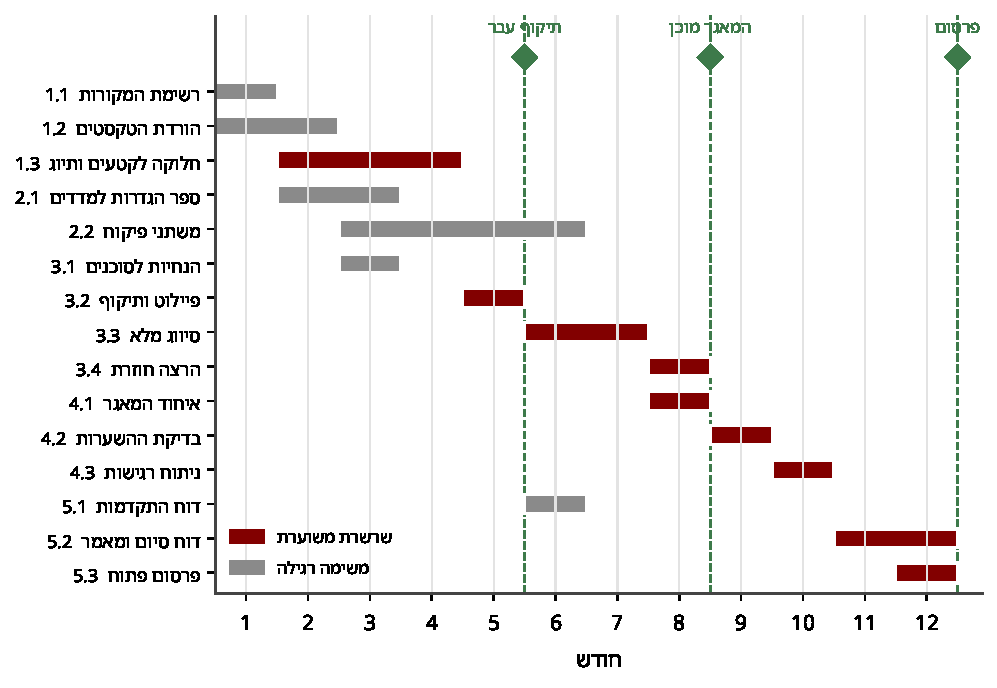
\includegraphics[width=0.92\textwidth]{figures/ch6-gantt.pdf}
  \caption{תרשים גאנט: 12 חודשים, שרשרת התלויות המשוערת באדום ושלוש אבני דרך בירוק}
  \label{fig:gantt}
\end{figure}

\paragraph{משמעות התלויות.} ציר החודשים הוא ברזולוציה גסה, וחלק מן המשימות נמסרות באצוות: רשימת ליבה מאושרת בחודש 1 מאפשרת התחלת הורדה, וטיוטת קידוד מאושרת מאפשרת הכנת הנחיות ואיסוף משתני פיקוח לפני סיום כל העדכונים. בחודש 8 בדיקת העקביות תסתיים לפני אישור המאגר; בחודש 12 הגרסה הסופית תינעל לפני הפרסום. אין להסיק מן החפיפה שכל תוצר סופי זמין בתחילת החודש. זו תוכנית תלויות מקדימה ולא חישוב \en{CPM} מלא; תאריכי המסירה, משכי העבודה ומרווחי הביטחון ייקבעו בתוכנית שבועית לפני ביצוע.

\paragraph{הנתיב הקריטי המשוער.} האדום מסמן שרשרת משוערת של אבני דרך תלויות: חלוקת הטקסטים לקטעים, הפיילוט והתיקוף, הסיווג המלא, בדיקת העקביות, איחוד המאגר, בדיקת ההשערות, ניתוח הרגישות, כתיבת דוח הסיום והפרסום. ההנחה היא שקיימת גמישות מסוימת במשימות כגון איסוף משתני הפיקוח ודוח ההתקדמות; היקפה טרם חושב, וכל שינוי ייבחן מול מועדי המסירה.

\paragraph{שלוש אבני הדרך.}
\begin{itemize}
  \item \textbf{סוף חודש 5: התיקוף עבר.} זו אבן הדרך החשובה ביותר: אם סיווגי המודל אינם עומדים ביעד של 85\%, אי אפשר להמשיך לסיווג המלא. לכן היא ממוקמת מוקדם, כשעוד יש זמן לתקן (פרק~\ref{ch:risks}).
  \item \textbf{סוף חודש 8: המאגר מוכן.} כל הנתונים – הסיווגים ומשתני הפיקוח – נמצאים במאגר אחד ועברו בדיקת שלמות (\en{REQ-DATA-01}).
  \item \textbf{סוף חודש 12: פרסום.} דוח הסיום, המאמר, והקוד והנתונים בגישה פתוחה.
\end{itemize}

\paragraph{מה קורה אם הפיילוט נכשל.} התיקוף נמצא על הנתיב הקריטי, ולכן כישלון שלו יעכב את כל המחקר. זו הסיבה שהוא ממוקם מוקדם ככל האפשר – בחודש החמישי, ולא לקראת הסוף. סבב תיקון ומבחן חדש צפויים לדרוש כחודש נוסף לפי הנחת התכנון. משום שהמשימה קריטית, אין בתוכנית מרווח שמבטיח ספיגה אוטומטית של העיכוב. במקרה כזה תוגש תוכנית מעודכנת: הקבלה של כתיבה וניתוח, צמצום היקף מאושר או הארכת לוח הזמנים. התוכנית לצמצום העיכוב הזה, ותוכנית המגירה אם גם הסבב השני ייכשל, מפורטות בפרק~\ref{ch:risks}.


\section{תקציב ומשאבים}
\label{sec:wp-budget}

טבלה~\ref{tab:budget} מציגה תקציב תכנון, לא הצעת מחיר מספק ולא הוצאה שכבר בוצעה. שני החוקרים מתוכננים להשקיע עשר שעות בשבוע כל אחד במשך 48 שבועות, בסך 960 שעות. לצורך השוואת חלופות בלבד הוערכה שעת חוקר ב־80 ש״ח ושעת מומחה ב־250 ש״ח. אלה הנחות תקציביות לאישור. הקצאת 70 שעות מומחה כוללת פיתוח קידוד, תיוג 450 קטעים, בדיקה כפולה של 60 קטעים והכרעת מחלוקות; היא תיבחן מחדש לאחר מיני־הפיילוט.

\begin{table}[htbp]
  \centering
  \caption{תקציב תכנון בש״ח לפי הנחות משאבים}
  \label{tab:budget}
  \small
  \begin{tabular}{p{48mm}p{51mm}r}
    \toprule
    \textbf{רכיב} & \textbf{בסיס החישוב} & \textbf{עלות} \\
    \midrule
    זמן שני החוקרים & \en{960 $\times$ 80} & \en{76,800} \\
    מומחה ותיוג נוסף & \en{70 $\times$ 250} & \en{17,500} \\
    שירותי מודלים & תקרת הקצאה לתכנון & \en{1,000} \\
    אחסון וגיבוי & תקרת הקצאה לתכנון & \en{1,000} \\
    \midrule
    סה״כ לפני עתודה & סכום ארבעת הרכיבים & \en{96,300} \\
    עתודה & \en{15\%} מהסכום & \en{14,445} \\
    \textbf{סה״כ כלכלי} & כולל זמן החוקרים & \en{110,745} \\
    \bottomrule
  \end{tabular}
\end{table}

אם זמן החוקרים ניתן כתרומה אקדמית ללא תשלום, התקציב הכספי המתוכנן הוא 19,500 ש״ח לפני עתודה ו־22,425 ש״ח אחריה. אין בכך התחייבות למימון. לפני שלב הביצוע יאושרו זמינות המומחה, התעריפים והתקרה. שינוי בשעות התיוג או שימוש בקידוד ידני יחייב עדכון משותף של התקציב ולוח הזמנים.

עלות המודל תיאמד מתוך 50 קטעי המיני־פיילוט: מספר טוקני קלט ופלט ממוצע לקטע, כפול מספר הקטעים, ההרצות וסוכני הבדיקה, במחירי המודל שנבחר ביום האישור. ב־80\% מניצול תקרת 1,000 הש״ח תופסק הרצה חדשה עד לבחינה מחדש. יעד של 2,000 קטעים מתויגים נשאר בתוקף גם אם חלק מהתיוג יועבר למסלול ידני; הקטנתו מחייבת אישור שינוי דרישה.

\input{chapters/07-risks}
% ============================================================
% chapters/08-summary.tex -- פרק 8: סיכום – מוכנים לשלב הביצוע
% Content only. All design comes from template.cls.
% Figure: figures/ch8-next-steps.tex (TikZ)
% ============================================================

\chapter{סיכום: מוכנים לשלב הביצוע}
\label{ch:summary}

\paragraph{ממצאי ההכנה.} הדוח מציע לבחון את הקשר בין התנצרות, השתלבות הכנסייה ויציבות מדינית באמצעות השוואה מדידה של המערב הרומי, המזרח והממלכה הפרנקית. בספרות שנכללה בסקירה לא זוהתה השוואה התואמת בדיוק את המדדים המוצעים; זהו פער במסגרת הסקירה, ולא הוכחה שאין מחקר קודם בנושא (פרקים~\LR{\ref{ch:problem}--\ref{ch:literature}}). הכלים שנסקרו מספקים חלק מן התשתית, אך זמינות המקורות והיתר השימוש בכל מהדורה ייבדקו לפני איסוף הקורפוס (פרק~\ref{ch:market}). מטריצת ההחלטה מעדיפה שילוב של מאגר נתונים וניתוח טקסט בעזרת \en{AI}, עם מבחן מומחה חתום ונפרד מקטעי הפיתוח. בדיקת הרגישות תומכת ביציבות ההעדפה תחת ההנחות שנבדקו, ואינה מדד להצלחת המחקר בעתיד (פרק~\ref{ch:alternatives}).

\paragraph{המוכנות לשלב הבא.} שבע הדרישות כוללות ערכי יעד ושיטות אימות. התוכנית כוללת חמש חבילות עבודה, שלוש אבני דרך ותקציב תכנון לצורך ההצעה: כ־111 אלף ש״ח כלכליים, וכ־22 אלף ש״ח במזומן אם זמן החוקרים ניתן כתרומה אקדמית. זהו אומדן ולא התחייבות למימון. המעבר לביצוע מותנה בזמינות מומחים ומקורות ובאישור התוכנית (פרק~\ref{ch:workplan}). הפחתת ארבעת הסיכונים הקריטיים היא תחזית תכנון המותנית בפעולות המנע; הכיסוי, הדיוק והעלויות טרם נמדדו (פרק~\ref{ch:risks}).

\paragraph{שלוש הפעולות המיידיות.} לאחר אישור הדוח יבוצעו הפעולות שבאיור~\ref{fig:next-steps}: גיוס מומחה ומומחה גיבוי וקביעת מועד התיקוף; הכנת ספר קידוד ורשימת מקורות; ומיני־פיילוט נפרד על 50 קטעים לבדיקת זמינות, עלות ואיכות ראשונית. מיני־הפיילוט אינו מחליף את מבחן 300 הקטעים החתום. המחקר עצמו לא בוצע במסגרת מטלה זו.

\begin{figure}[htbp]
  \centering
  \input{figures/ch8-next-steps}
  \caption{שלוש הפעולות המיידיות לאחר אישור הדוח}
  \label{fig:next-steps}
\end{figure}

\begin{keybox}{בחזרה לאוגוסט 410}
כשהוויזיגותים נכנסו לרומא, בני התקופה מיהרו לשאול מי אשם: האלים שננטשו, או האל החדש. המחקר המוצע לא מבקש להכריע מי צדק אז, אלא לאפשר לבדוק את השאלה באופן שיטתי – בנתונים, בשיטה שאפשר לשחזר, ובאותם מדדים לשלוש מדינות שבחרו באותה דת והגיעו לגורלות שונים כל כך.
\end{keybox}


% ---------- References ----------
\printbibliography

\end{document}
